\subsection{Covariant and Contravariant Vectors}

For a chosen set of variables $u^i$, we can define the constant $u^i$ surfaces and the curves that $u^i$ increase. The surfaces will have a normal vector of $\Vec{\nabla u^i}$. And the direction of the curves are $\cfrac{\partial \Vec{R}}{\partial u^i}$. Notice these new parameters and the coordinates that define them don't need to be orthogonal or unit vectors.
\begin{figure}[H]
    \centering
    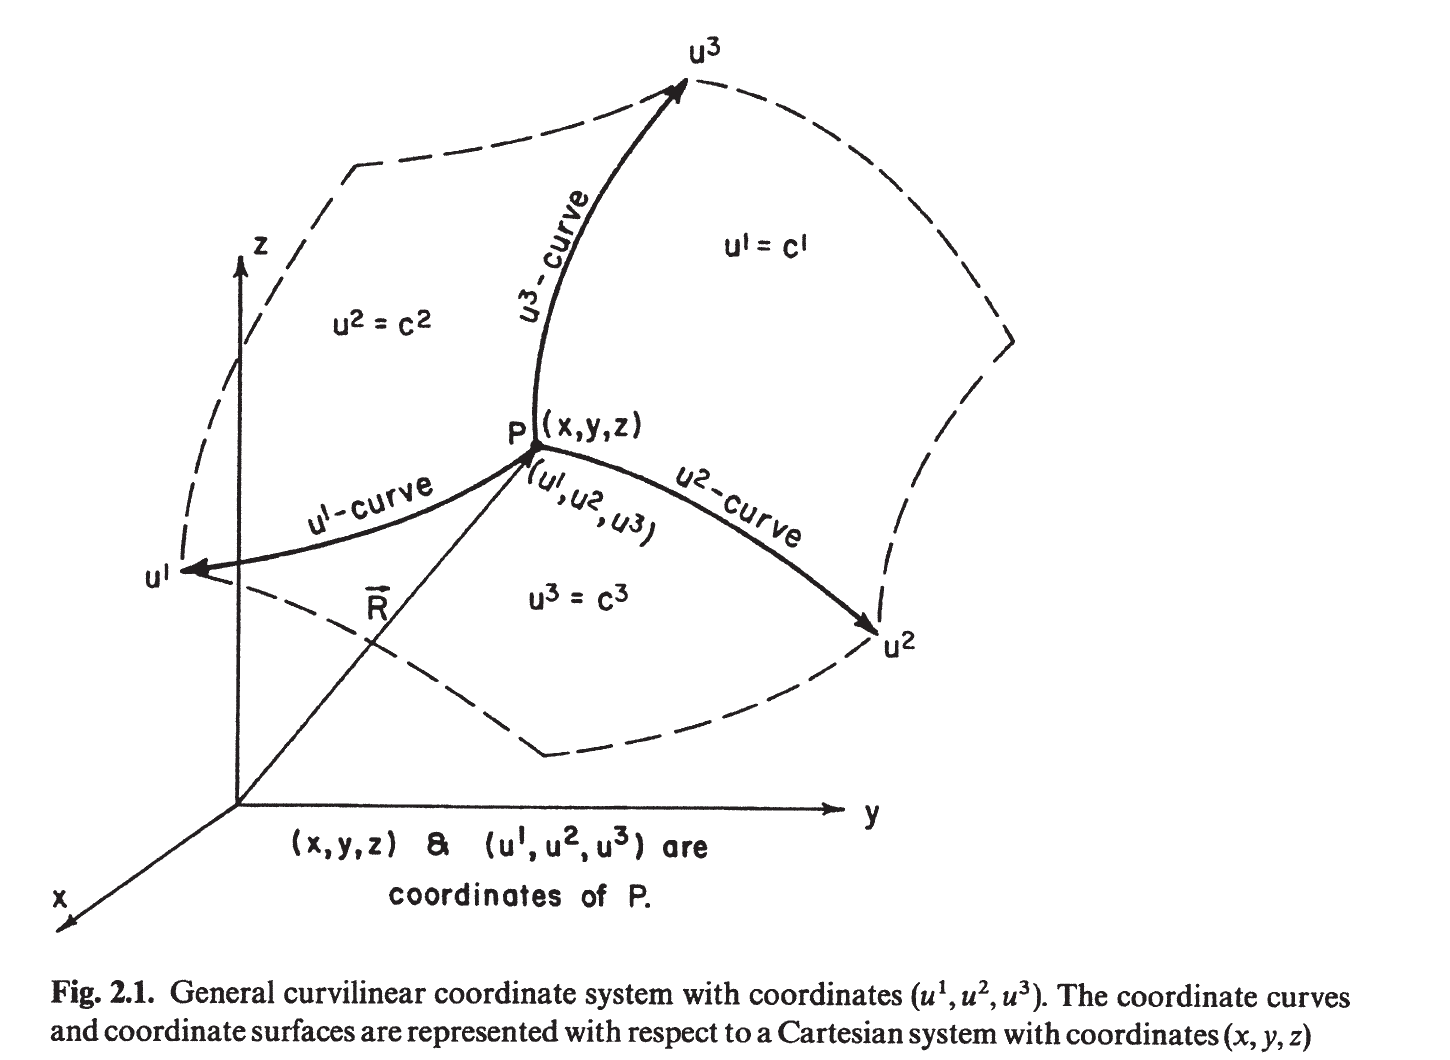
\includegraphics[width=11cm]{d'haaseleer-coordinates.png}
    \caption{General curvilinear coordinate system \cite{dhaeseleer_flux_2012}}
\end{figure}
The differential change of $u^i$ can be written as,
\begin{equation}
    du^i = \nabla u^i \cdot d\textbf{R}
\end{equation}
Since $\Vec{R}$ can be written as $\Vec{R}(u^1, u^2, u^3)$, we have,
\begin{align}
    d\textbf{R} = \sum_{j=1}^3 \cfrac{\partial \Vec{R}}{\partial u^j}du^j \hspace{.6cm} &\Rightarrow \hspace{.6cm} du^i = \nabla u^i \cdot \sum_{j=1}^3 \cfrac{\partial \Vec{R}}{\partial u^j}du^j \\
    du^i = \nabla u^i \cdot \cfrac{\partial \Vec{R}}{\partial u^i}du^i \hspace{.6cm} &\Rightarrow \hspace{.6cm} \nabla u^i \cdot \cfrac{\partial \Vec{R}}{\partial u^i} = \delta_j^i
\end{align}
From now on, we will use covariant and contravariant vectors with superscripts and subscripts,
\begin{align}
    \textbf{Contravariant: }& \hspace{1cm} \e_i = \cfrac{\partial \Vec{R}}{\partial u^i} \\[.5cm]
    \textbf{Covariant: }& \hspace{1cm} \e^i = \nabla u^i \\[.5cm]
    &\e^i \cdot \e_i = \delta_j^i \begin{cases}
        1 &\text{for } i=j\\
        0 &\text{otherwise}
    \end{cases}
\end{align}
And the transformation from these two sets of vectors is,
\begin{equation}
    \e^1 = \cfrac{\e_2 \times \e_3}{\e_1 \cdot (\e_2 \times \e_3)} \hspace{2cm} \e_1 = \cfrac{\e^2 \times \e^3}{\e^1 \cdot (\e^2 \times \e^3)}
\end{equation}
Since these are reciprocal sets of vectors, a vector P can be written as,
\begin{align}
    &\mathbf{P} =  (\mathbf{P} \cdot \e_1) \e^1 + (\mathbf{P} \cdot \e_2) \e^2 + (\mathbf{P} \cdot \e_3) \e^3 \\
    \text{or } &\mathbf{P} =  (\mathbf{P} \cdot \e^1) \e_1 + (\mathbf{P} \cdot \e^2) \e_2 + (\mathbf{P} \cdot \e^3) \e_3 \\
    \text{we will use } P_i =  \mathbf{P} \cdot \e_i \hspace{.6cm}&\text{and }\hspace{.6cm} P^i =  \mathbf{P} \cdot \e^i \\
    \mathbf{P} =  P_1 \e^1 + P_2 \e^2 + P_3 \e^3 \hspace{.6cm}&\text{or }\hspace{.6cm} \mathbf{P} =  P^1 \e_1 + P^2 \e_2 + P^3 \e_3 
\end{align}
\footnote{This seems a bit counter-intuitive because, in orthonormal coordinates systems (that are the most used coordinates), you should take the dot product of the vector with the basis vector you want to find the component of.}For example in cartesian coordinates, $P_x = \mathbf{P} \cdot \hat{x}$ and \(\mathbf{P} = (\mathbf{P} \cdot \hat{x}) \hat{x} + (\mathbf{P} \cdot \hat{y}) \hat{y} + (\mathbf{P} \cdot \hat{z}) \hat{z}\). Note that in orthonormal coordinate systems, the contravariant and covariant basis vectors are the same, implying \(\mathbf{e}^i = \mathbf{e}_i = \mathbf{e}_i / \Vert \mathbf{e}_i \Vert\), so they are self-reciprocal.

\begin{figure}[H]
    \centering
    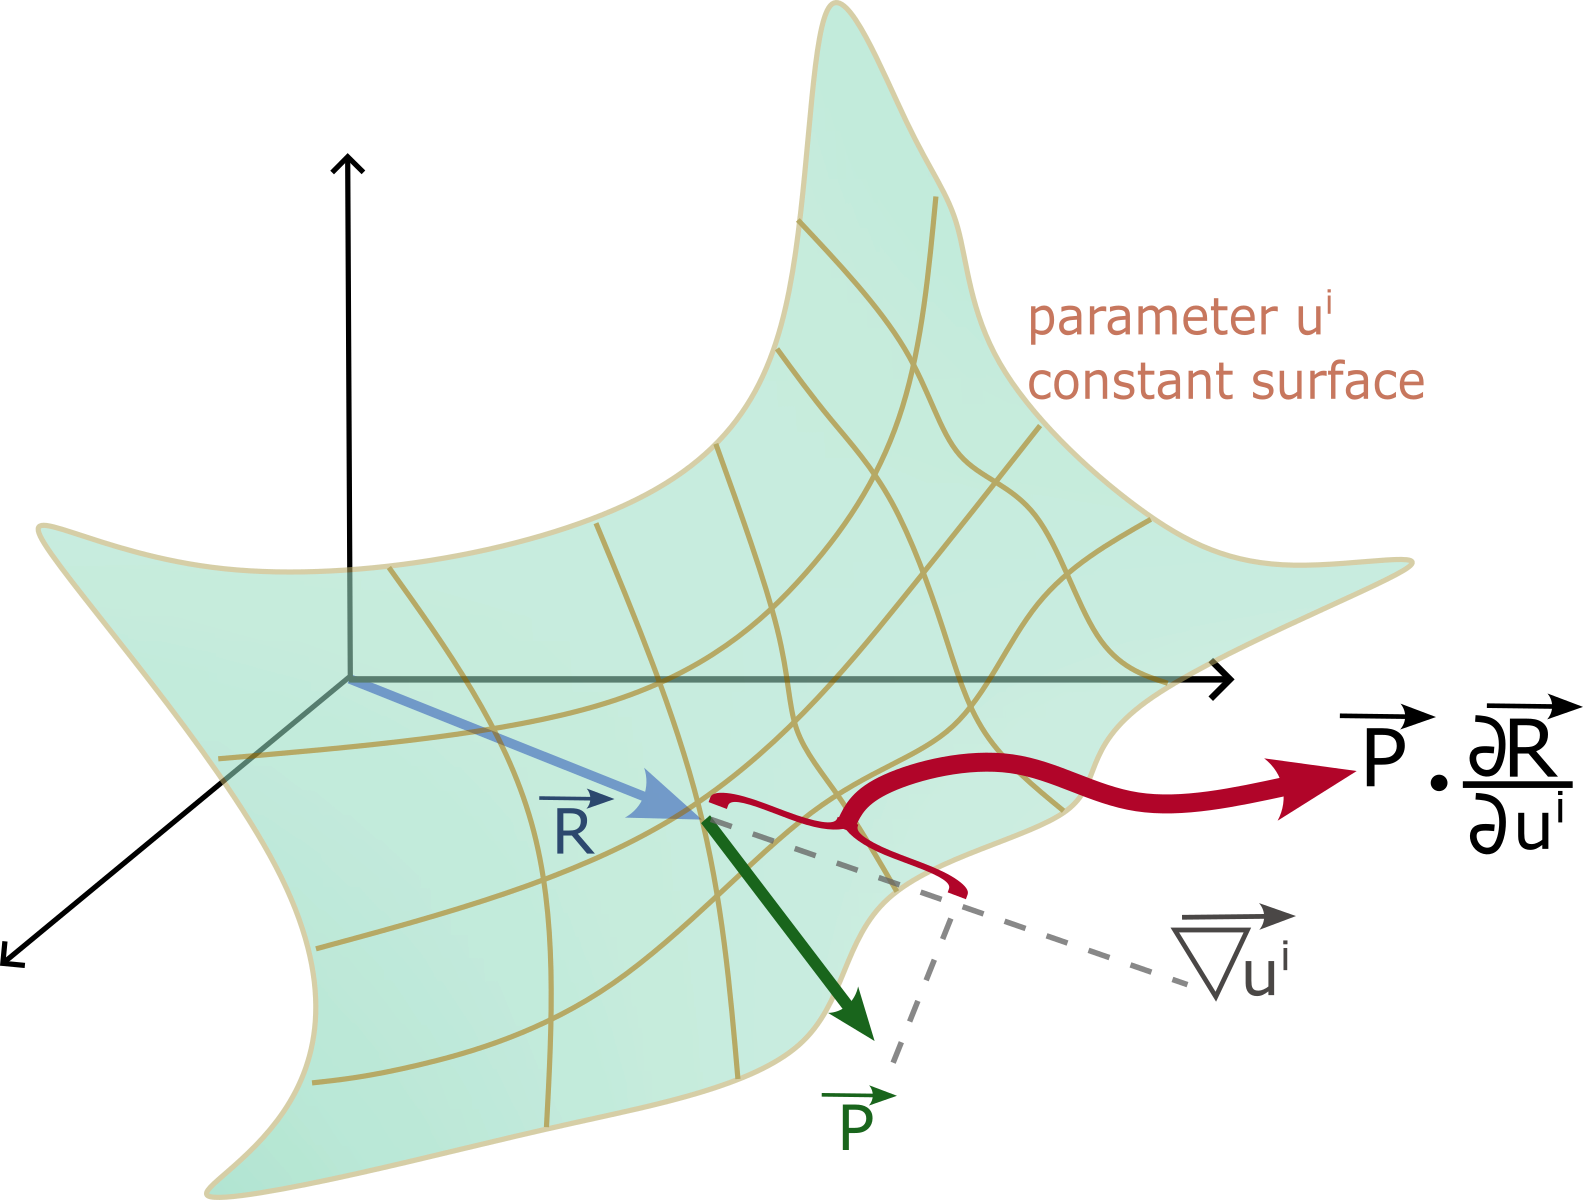
\includegraphics[width=9cm]{surface-covariant.png}
\end{figure}

Now, back to the stellarators. We will use contravariant basis vectors for the $\rho, \theta$  and $\zeta$ as follows,
\begin{equation}
    \e_i = \cfrac{\partial \Vec{R}}{\partial u^i} = \cfrac{\partial }{\partial u^i} (R\hat{R} + Z\hat{Z})
\end{equation}
In general, the derivative of the unit vectors is 0, but only the $\zeta$ contravariant vector has an exception.
\begin{equation}
    \e_\zeta = \cfrac{\partial }{\partial \zeta} (R\hat{R} + Z\hat{Z}) 
    = \cfrac{\partial R}{\partial \zeta}\hat{R} + R\cfrac{\partial \hat{R}}{\partial \zeta} + \cfrac{\partial Z}{\partial \zeta}\hat{Z} + Z\cfrac{\partial \hat{Z}}{\partial \zeta}
    = \cfrac{\partial R}{\partial \zeta}\hat{R} + R\hat{\phi} + \cfrac{\partial Z}{\partial \zeta}\hat{Z}
\end{equation}
We got an additional $R\hat{\phi}$ term due to the partial derivative of $\hat{R}$ with respect to $\zeta$. Using similar steps, one can get the full set of covariant basis vectors as follows,
\begin{equation}
    \e_\rho =  \begin{bmatrix}
        \partial_\rho R \\ 0 \\ \partial_\rho Z
    \end{bmatrix} \hspace{1cm}
    \e_\theta =  \begin{bmatrix}
        \partial_\theta R \\ 0 \\ \partial_\theta Z
    \end{bmatrix}\hspace{1cm}
    \e_\zeta =  \begin{bmatrix}
        \partial_\zeta R \\ R \\ \partial_\zeta Z
    \end{bmatrix}
\end{equation}
If you are confused about the basis vectors being different for each point, think about cylindrical or spherical coordinates. $\hat{\theta}$ and $\hat{\phi}$ change direction for every point in space. Since we use them a lot and they are orthogonal, we tend to ignore this fact. But in general, you can choose any random parameter that has defined constant surfaces. Then, you can create a covariant or contravariant basis using those parameters. For example, the spherical coordinates have constant surfaces as shown in Figure \ref{spherical-coord-planes}. the basis vectors are perpendicular to those surfaces. I hope this example didn't even confuse you about spherical and cylindrical coordinates. Give yourself some time, and read this a couple of times. I assure you it will make sense after some point.
\begin{figure}[H]
    \centering
    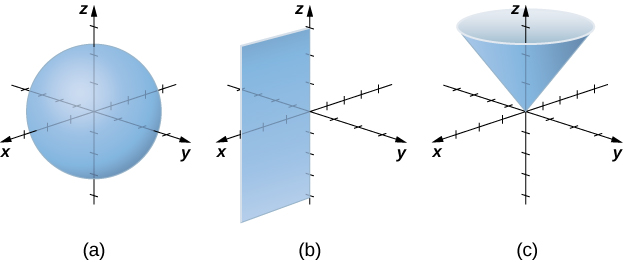
\includegraphics[width=10cm]{figures/spherical-coord-constant-planes.jpg}
    \caption{Surfaces of constant parameters (a) $\rho$, (b) $\theta$ and (c) $\phi$
    \cite{noauthor_57_2019}}
    \label{spherical-coord-planes}
\end{figure}

And, we will also need the Jacobian of this basis vectors that can be found by,
\begin{equation}
    \jac = \e_\rho \cdot (\e_\theta \times \e_\zeta) \hspace{1cm} \text{or } \hspace{1cm} \jac = \begin{vmatrix}
                    \partial_\rho R & \partial_\rho \phi & \partial_\rho Z \\
                    \partial_\theta R & \partial_\theta \phi & \partial_\theta Z\\
                    \partial_\zeta R & \partial_\zeta \phi & \partial_\zeta Z
                \end{vmatrix} 
\hspace{1cm} \text{or } \hspace{1cm} \frac{1}{\jac} = \e^\rho \cdot (\e^\theta \times \e^\zeta)
\end{equation}
\begin{equation}
    \begin{split}
        \jac &=  \begin{bmatrix} \partial_\rho R & 0 & \partial_\rho Z \end{bmatrix} \cdot
                \begin{vmatrix}
                    \hat{r} & \hat{\phi} & \hat{z} \\
                    \partial_\theta R & 0 & \partial_\theta Z\\
                    \partial_\zeta R & R & \partial_\zeta Z
                \end{vmatrix} \\[0.5cm]
                &=  \begin{bmatrix} \partial_\rho R & 0 & \partial_\rho Z \end{bmatrix}
                        \begin{bmatrix}
                            R \partial_\theta Z \\
                            \partial_\theta Z \partial_\zeta R - \partial_\theta R \partial_\zeta Z \\
                            R \partial_\theta R
                        \end{bmatrix} \\[0.5cm]
    \end{split}
\end{equation}
Finally, we get,
\begin{equation}
    \jac =  R \left( \dRr  \dZt +      
        \dRt  \dZr \right)   \label{jacobian}
\end{equation}
with Jacobian, we can rewrite transformations as,
\begin{align}
    \e^i \times \e^j = \varepsilon^{ijk} \frac{\e_k}{\jac} \label{icrossj} \\[.5cm]
    \e_i \times \e_j = \varepsilon^{ijk} \jac \e^k
\end{align}
\begin{equation}
    \e^1 = \cfrac{\e_2 \times \e_3}{\jac} \hspace{2cm} \e_1 = \jac (\e^2 \times \e^3)
\end{equation}

